\section{Systemarkitektur}
\label{ch:systemarkitektur}
I dette afsnit vil systemarkitekturen for projektet blive beskrevet. Systemarkitekturen tager udgangspunkt i dokumentationsdokumentet \textit{Arkitektur}, og for nærmere uddybning henvises der til det dokument.\\
Systemarkitekturen er udarbejdet på grundlag af kravspecifikationen, og systemet som beskrevet i projektbeskrivelsen.

Systemarkitekturen starter med funktionaliteten beskrevet i use casene, og udvider så beskrivelsen til at omfatte de elementer af systemet, som brugeren ikke interagerer med. Dette afsnit vil give et eksempel på, hvordan en use case er blevet behandlet i systemarkitekturen. Use casen, der vil blive gennemgået, vil være use case 2: \textit{Skibsfører slår automatisk hældningsregulering til}.

\begin{figure}[H]
\centering
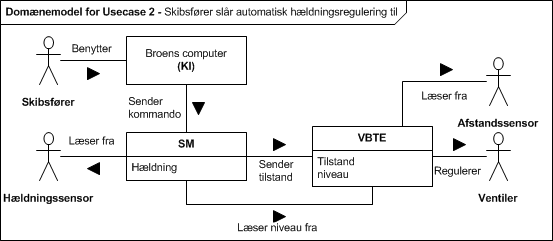
\includegraphics[scale=0.8]{billeder/Systemarkitektur/DM_UC2}
\caption{Domænemodel for use case 2}
\label{fig:dmuc2}
\end{figure}

\subsubsection{Relationen mellem elementer og aktører}
I domænemodellen på figur \ref{fig:dmuc2} beskrives relationen mellem systemets elementer og aktørerne. Disse enheder omdannes i klassediagrammet (figur \ref{fig:kduc2}) til konceptuelle klasser af en given type. Det ses at i use case 2 fungerer Kontrolinterfacet både som kontrolklasse og grænsefladeklasse. Kontrolinterfacet er kontrolklasse fordi det er initiativ- og beslutningstager til den efterfølgende udvikling i systemet. Både Kontrolinterfacet, Styringsmodulet og Vandballasttankenhederne fungerer som grænsefladeklasser, fordi alle tre klasser er i berøring med en aktør.\\

\begin{figure}[H]
\centering
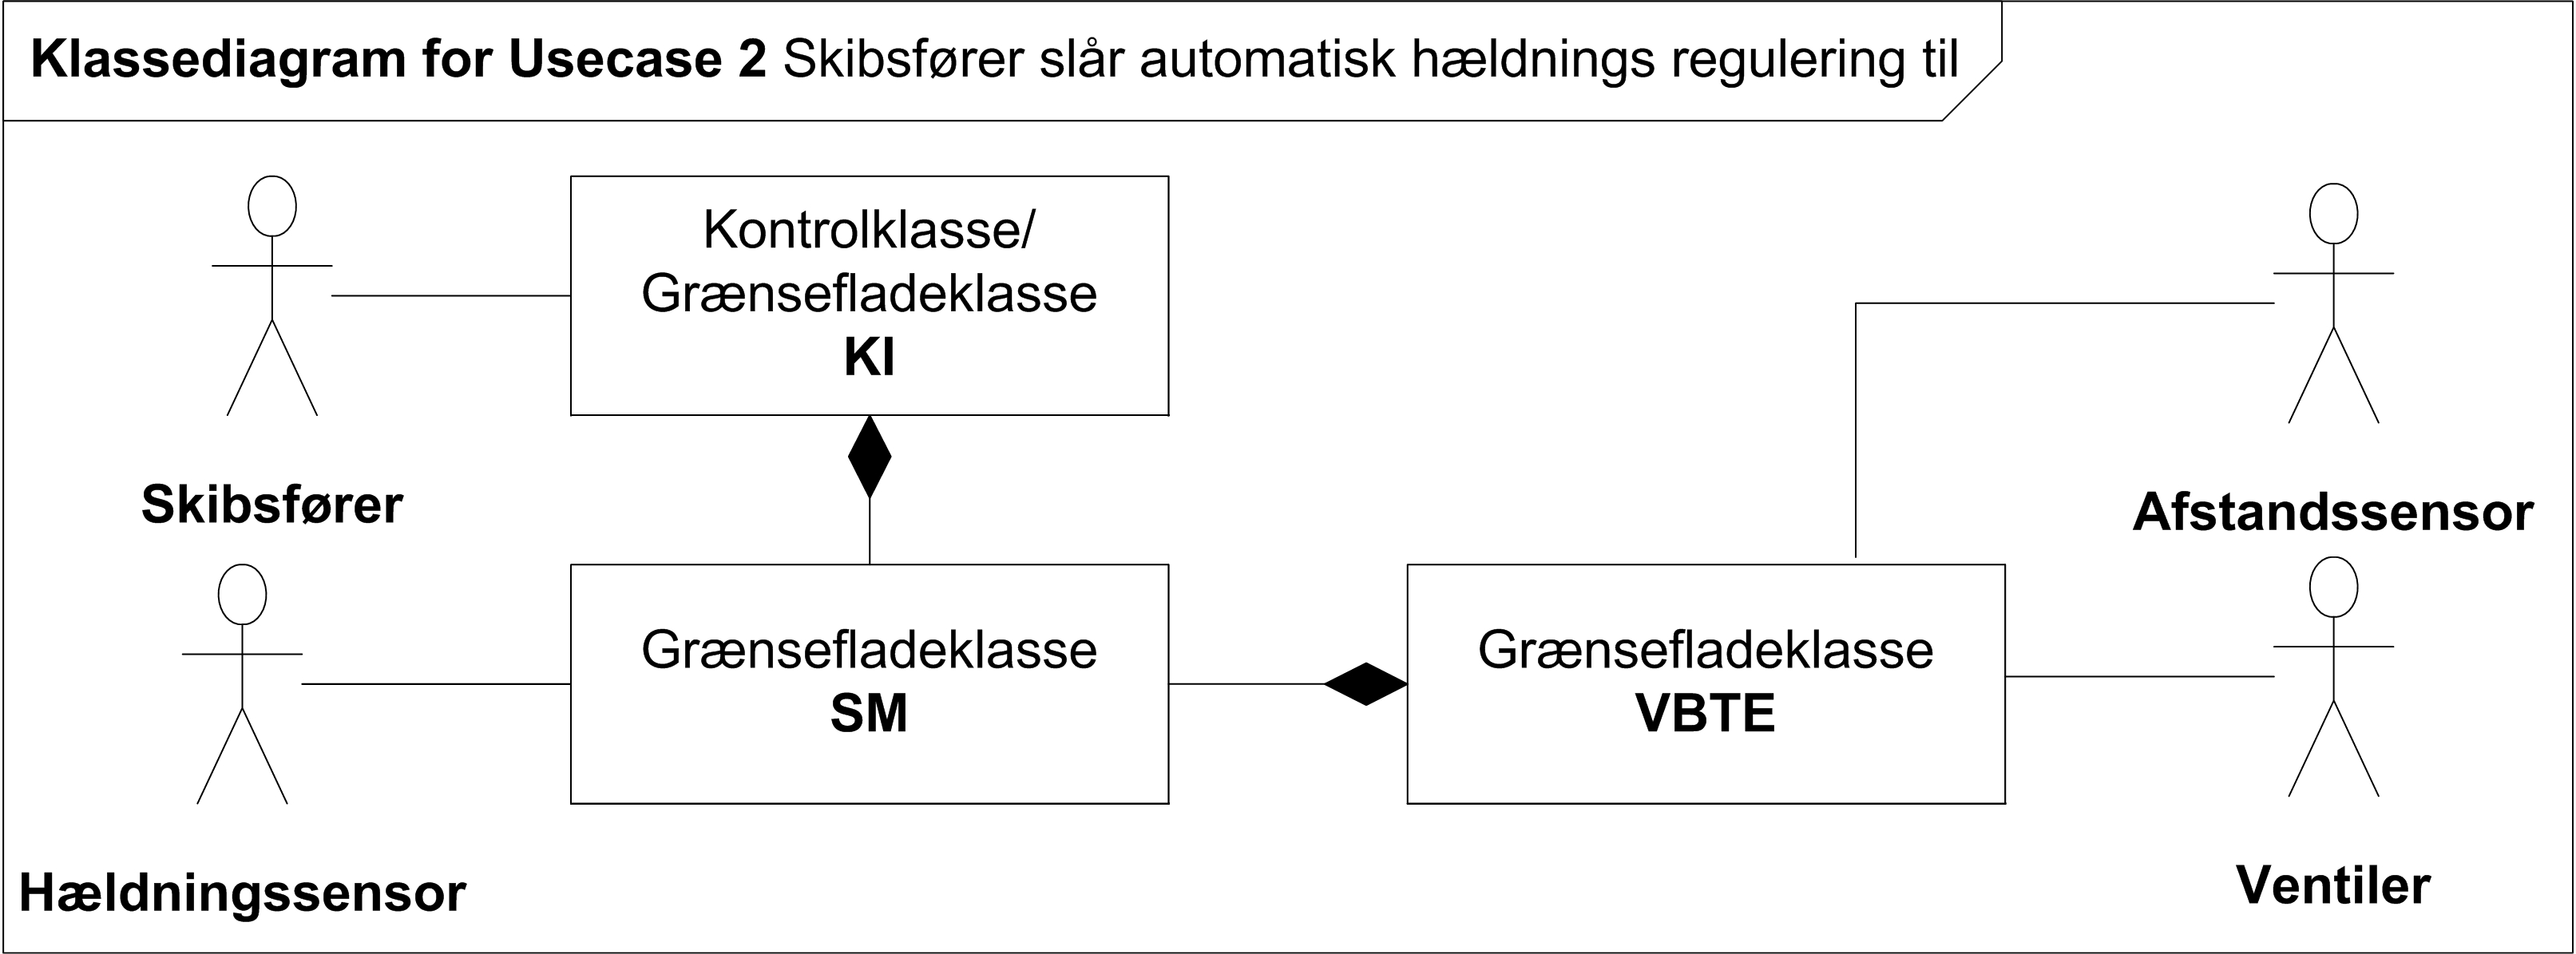
\includegraphics[scale=0.8]{billeder/Systemarkitektur/KD_UC2}
\caption{Klassediagram for use case 2}
\label{fig:kduc2}
\end{figure}


\subsubsection{Kommunikation og timing}
I sekvensdiagrammet (figur \ref{fig:sduc2}) beskrives kommunikationen og timingen imellem klasserne. Det ses at brugeren igangsætter processen, herefter videresender Kontrolinterfacet kommandoen og Styringsmodulet bekræfter modtagelsen. Styringsmodulet begynder så at regulere på vandniveauet i tankene ved hjælp af Vandballasttankenhederne. Reguleringen sker på grundlag af de målinger, der modtages fra hældningssensoren. Vandniveauet vil blive ved med at blive reguleret med det formål at opnå og derpå opretholde en hældning på nul grader.

\begin{figure}[H]
\centering
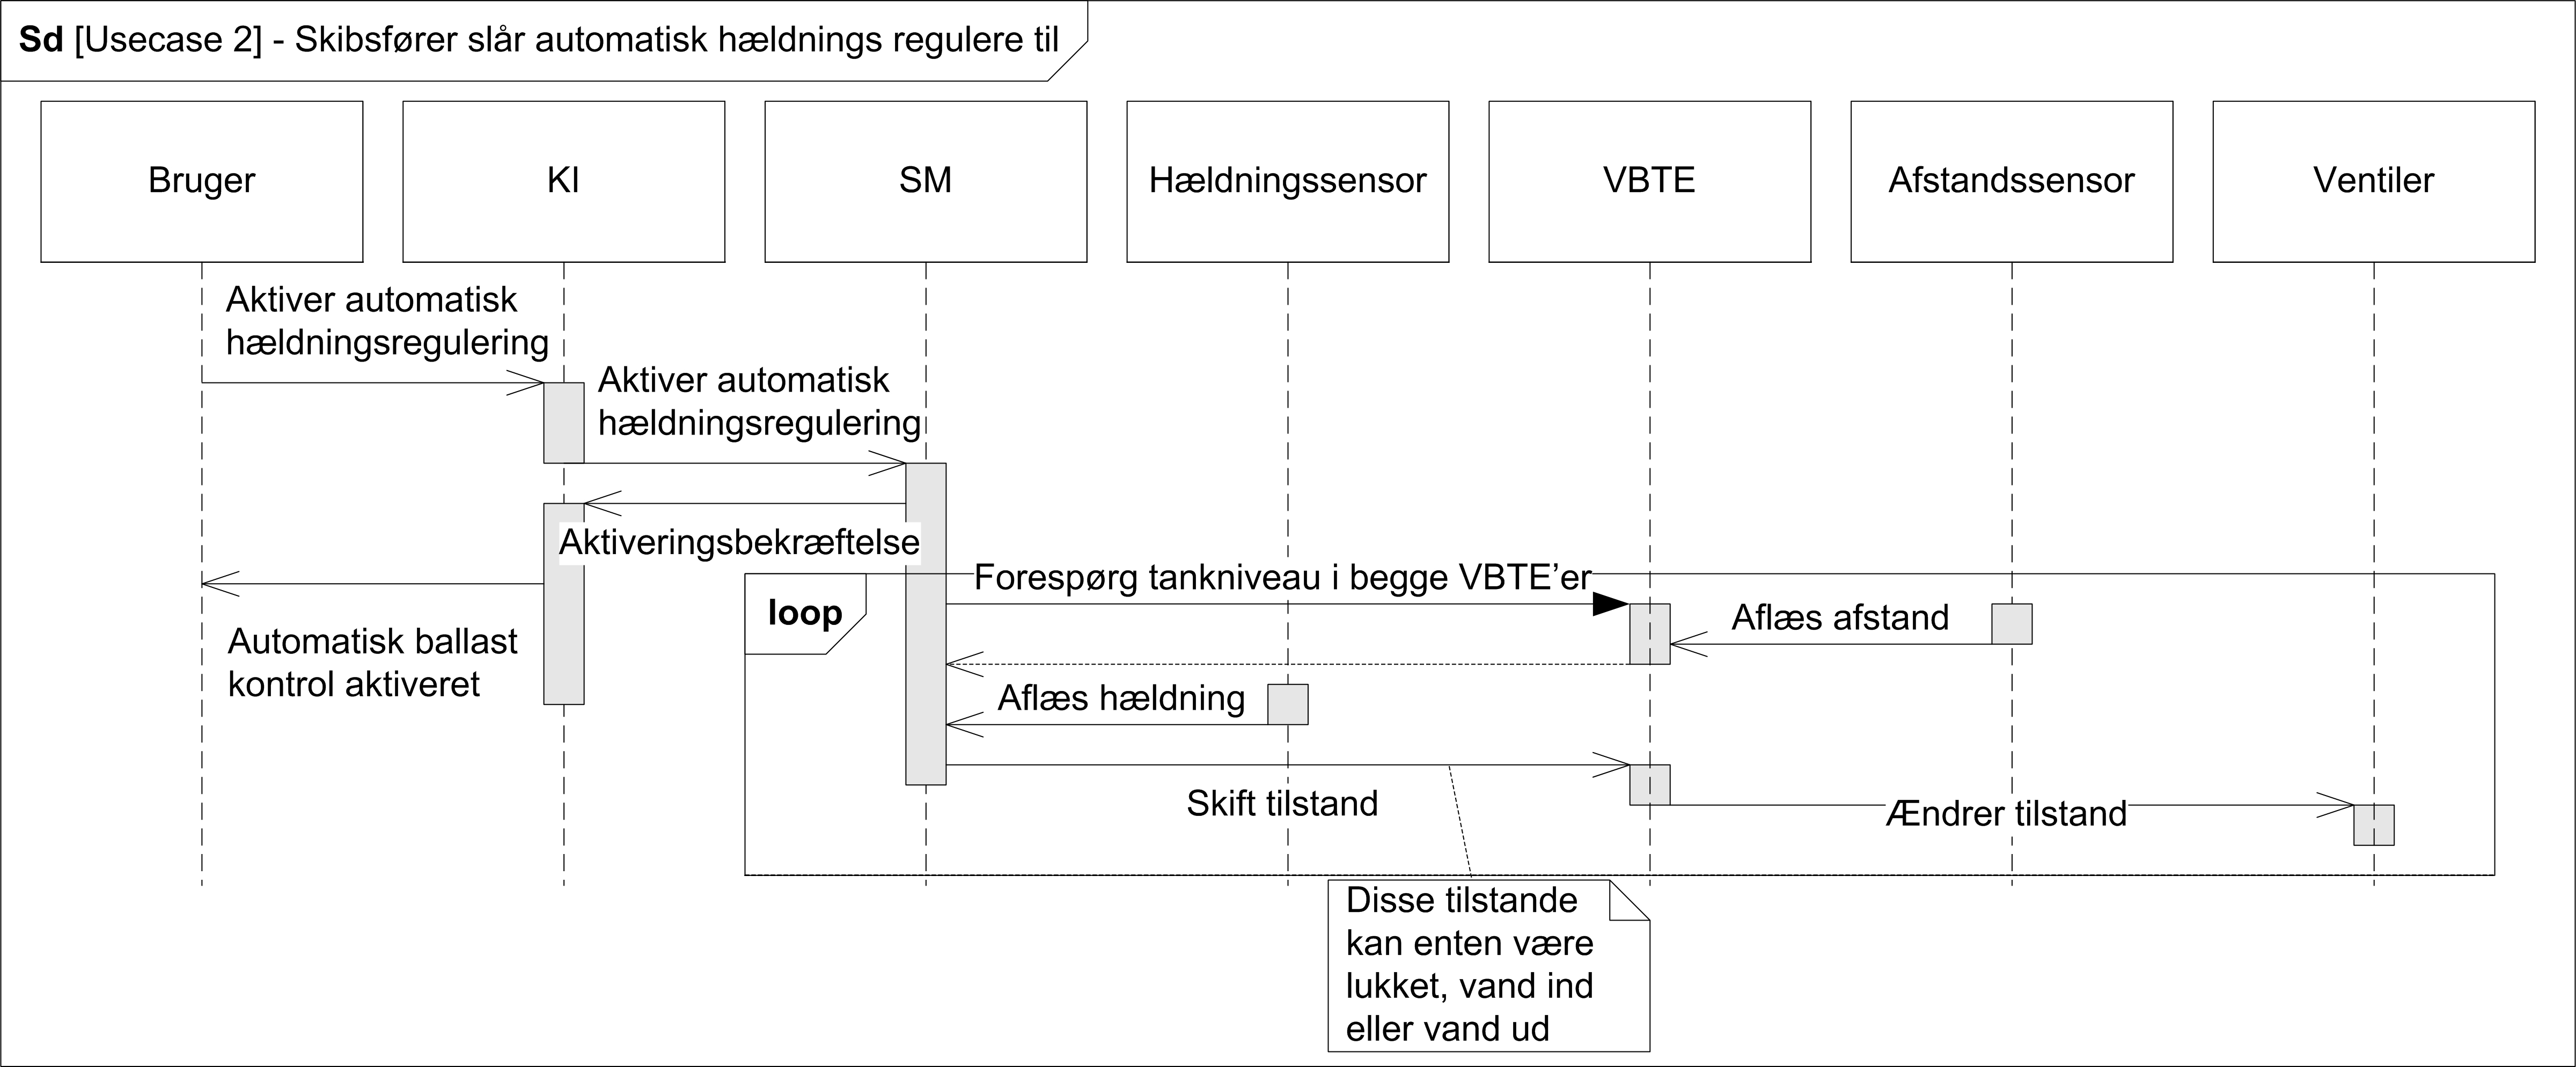
\includegraphics[scale=0.8]{billeder/Systemarkitektur/SD_UC2}
\caption{Sekvensdiagram for Use Case 2}
\label{fig:sduc2}
\end{figure}

\subsection{Stadier for konceptuelle klasser}
Når alle use cases er blevet bearbejdet som use case 2 er blevet i figur \ref{fig:dmuc2}, \ref{fig:kduc2} og \ref{fig:sduc2} har gruppen dannet state machines for de konceptuelle klasser i systemet. Her visualiseres hvilke stadier, klasserne har brug for at gennemgå i løbet af klassens levetid for at opfylde kravene sat i kravspecifikationen. Som et eksempel på en sådan state machine, vises state machinen for Styringsmodulet på figur \ref{fig:stm_sm}. \\

\begin{figure}[H]
\centering
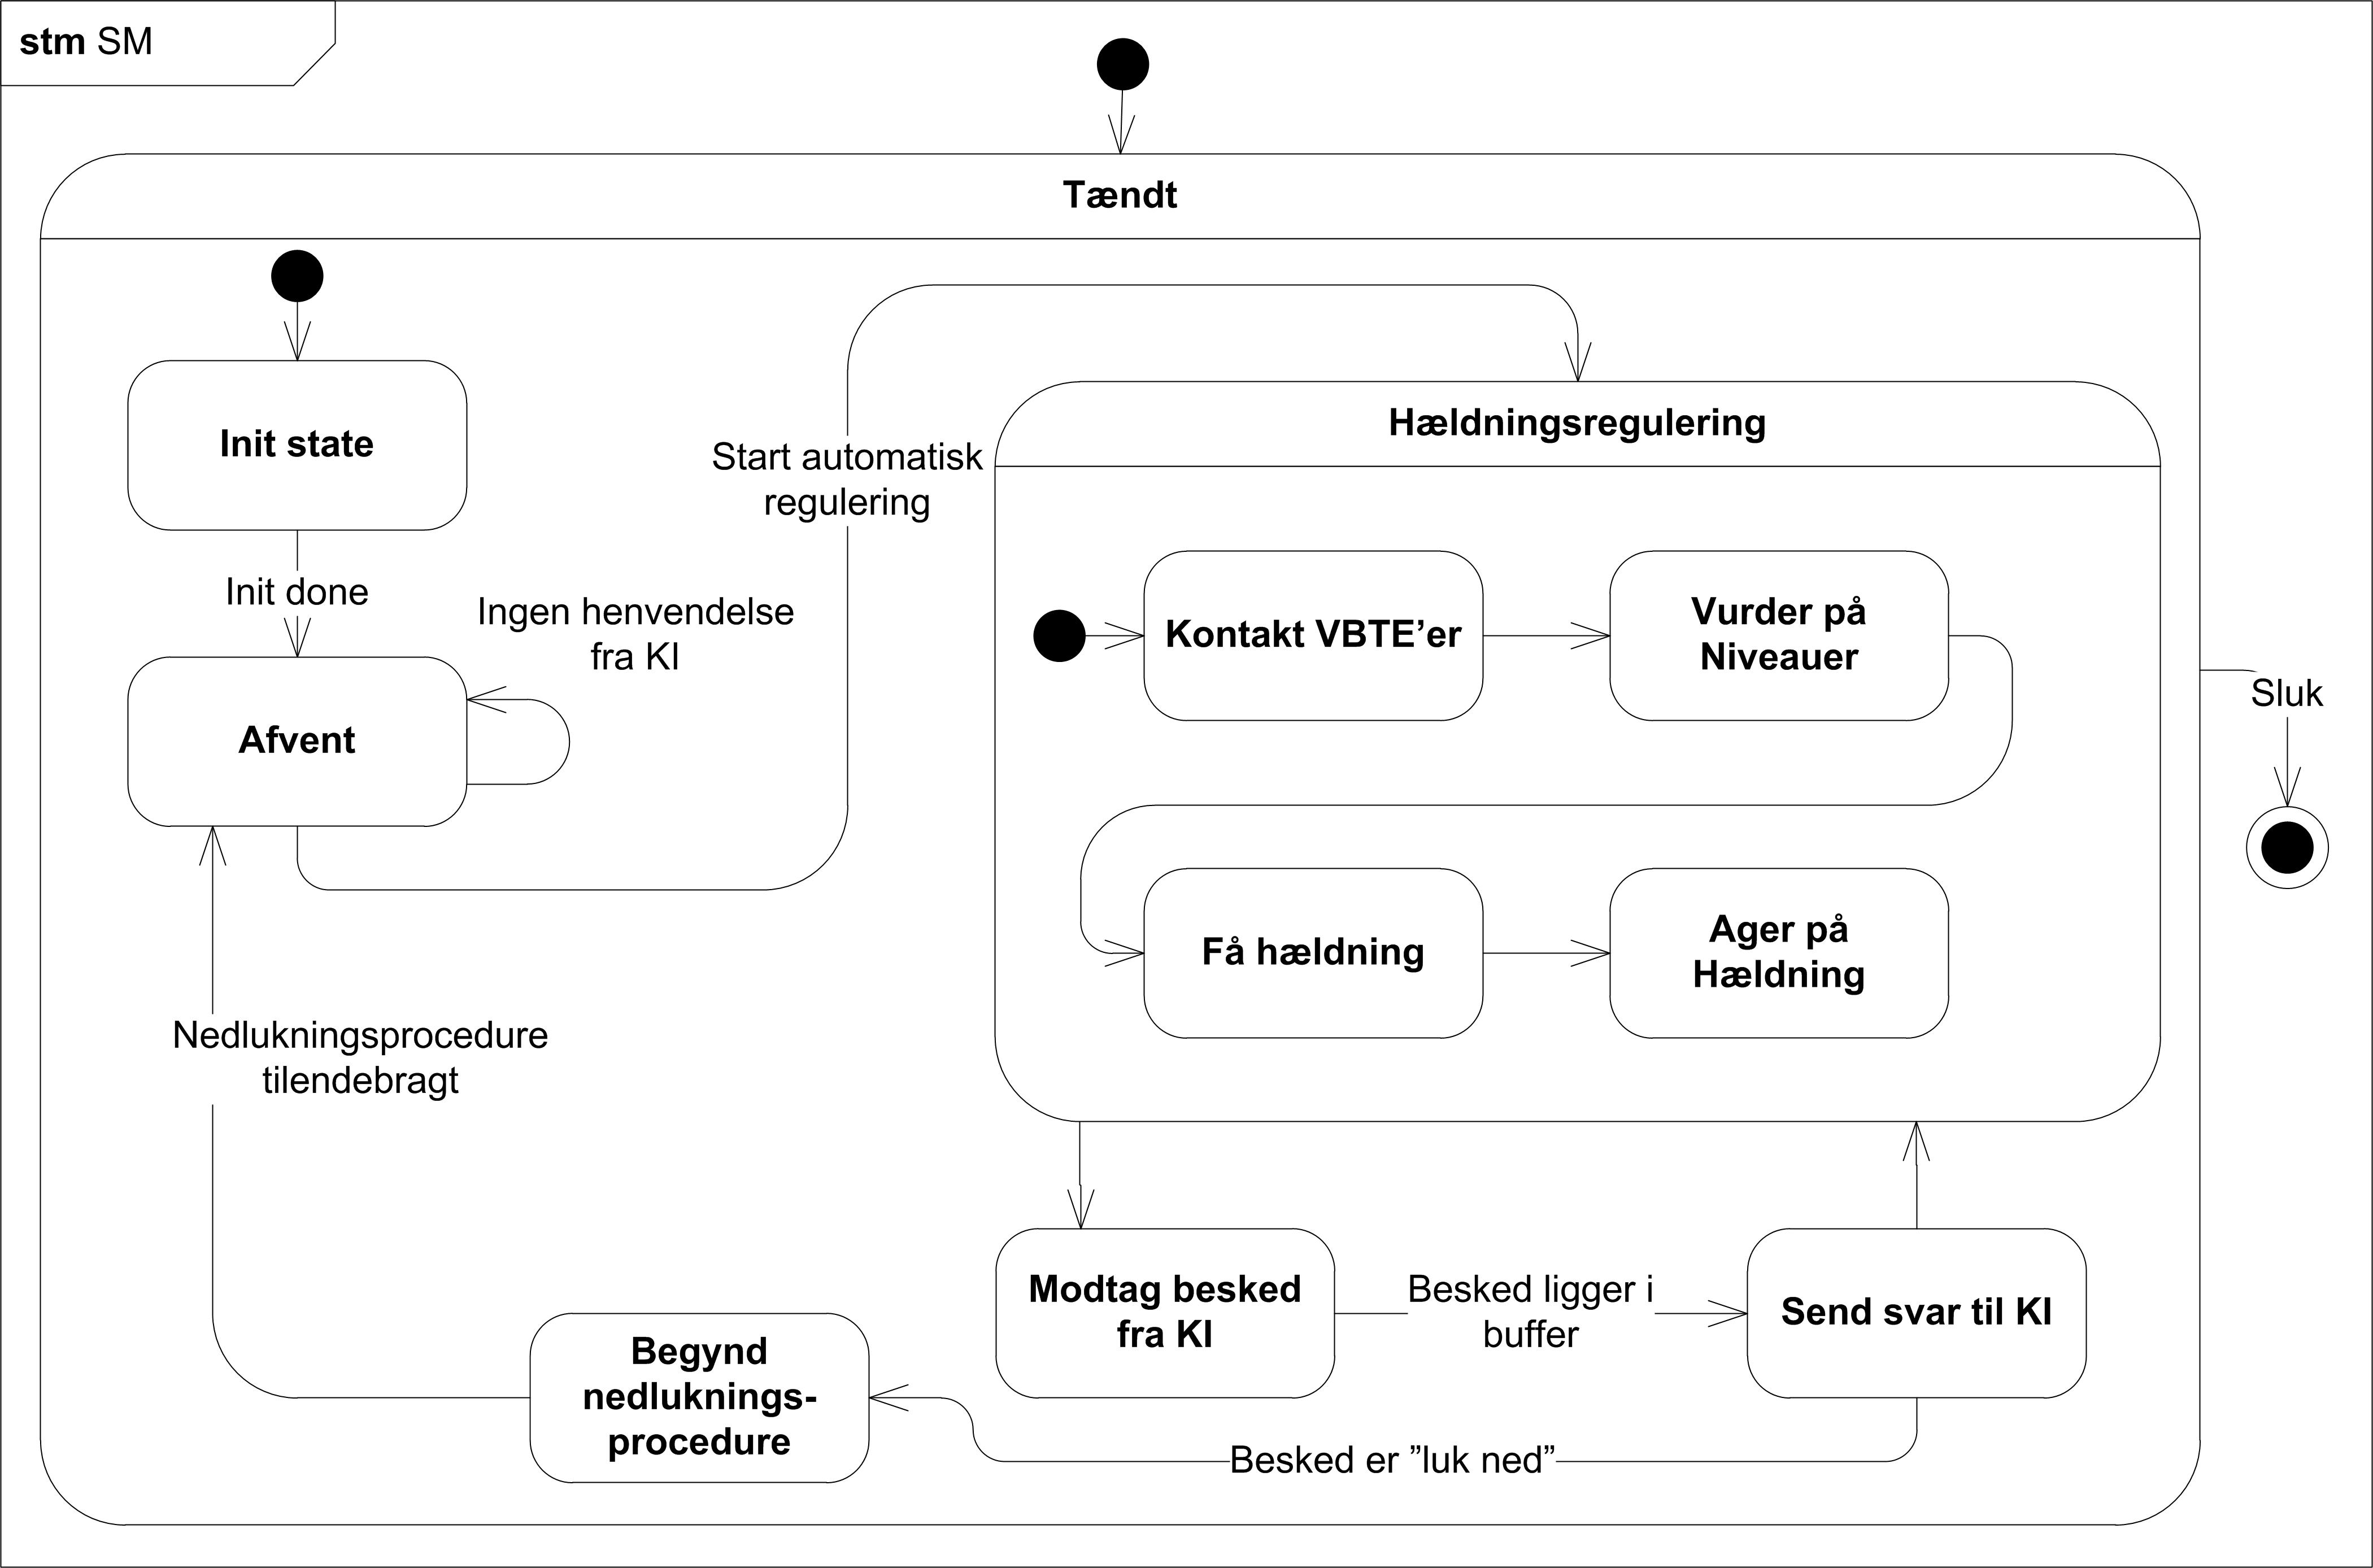
\includegraphics[width=0.7\textwidth]{billeder/Systemarkitektur/stm_sm}
\caption{State machine for Styringsmodulet}
\label{fig:stm_sm}
\end{figure}

Flowet i state machinen bygger på det beskrevne i sekvensdiagrammerne. Starten på use case 2 er et brugerinput til Kontrolinterfacet. Dette medfører en besked fra Kontrolinterfacet til Styringsmodulet. Styringsmodulet kan være i to forskellige stadier når den modtager beskeden:\\
Hvis programmet er nyopstartet, vil beskeden få Styringsmodulet ud af \textit{Afvent}-stadiet og til at aktivere automatisk hældningsregulering. Hvis programmet befinder sig i \textit{Hældningsregulering}-stadiet med reguleringstypen \textit{manuel}, vil beskeden fra Kontrolinterfacet få Styringsmodulet over i stadiet \textit{Modtaget besked fra KI}. Styringsmodulet besvarer beskeden med en aktiveringsbekræftelse, og returerner derpå til \textit{Hældningsregulering}-stadiet - nu med reguleringstypen \textit{automatisk}.

Dette var for use case 2. Styringsmodulets opførelse for alle use cases kan forudsiges på samme måde ud fra figur \ref{fig:stm_sm}. 

\subsubsection{Fra konceptuelle klasser til system}
Næste trin er, at omdanne de konceptuelle klasser til et regulært system. Nogle konceptuelle klasser kan grupperes, andre står for sig selv. Den fysiske opbygning af systemet, bliver så vist i et blokdefinitionsdiagram. Blokdefinitionsdiagrammet for systemet kan ses i figur \textit{\ref{fig:bdd_bros}}. Her ses det, at systemet ender ud med fire hovedblokke: Kontrolinterfacet, Styringsmodulet, Vandballasttankenhed og Database. De konceptuelle klasser, der ikke er endt som hovedblokke, er i stedet for blevet til underblokke af enten styringsmodulblokken eller vandballasttankenhedblokken.

\begin{figure}[htbp]
\centering
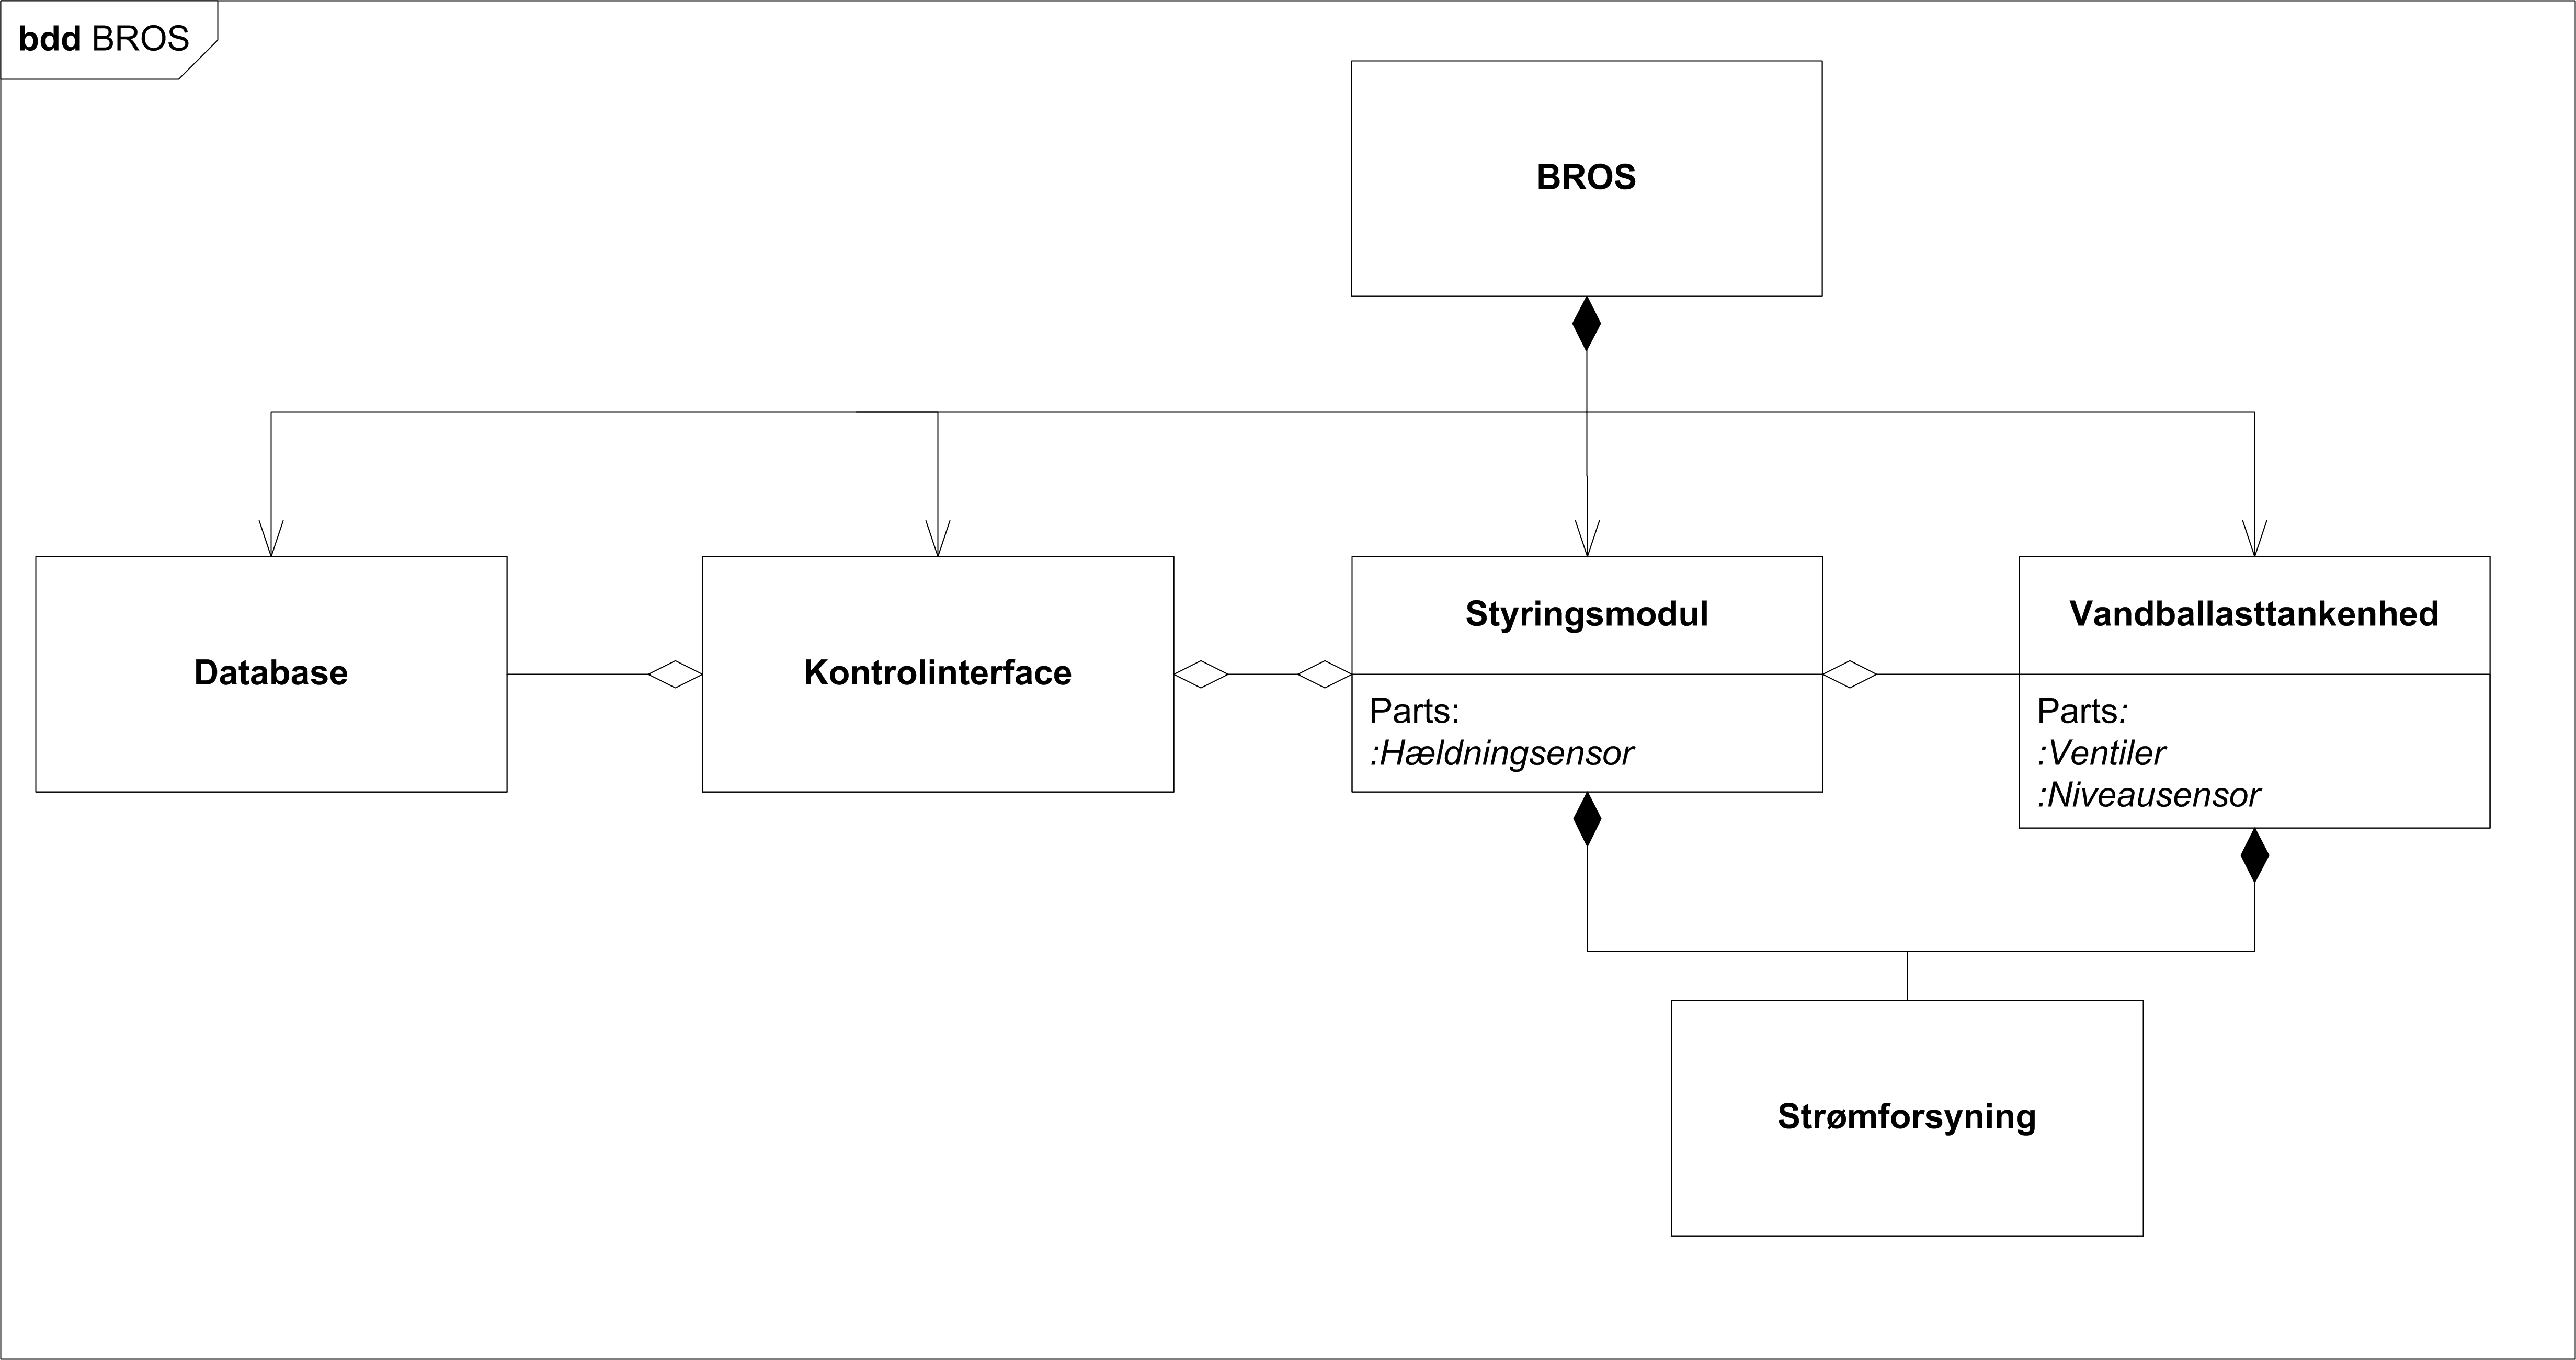
\includegraphics[scale=0.5]{billeder/Systemarkitektur/bdd_bros}
\caption{Blokdefinitionsdiagram for systemet}
\label{fig:bdd_bros}
\end{figure}

\subsubsection{Kommunikationsveje i systemet}
Herefter er opgaven to-delt. Kommunikationsvejene skal kortlægges både internt mellem blokkene og for inputs og outputs af systemet. Begge dele gøres i et internt blokdiagram. Det interne blokdiagram for systemet kan ses i figur \ref{fig:idb_bros}. Her angives det også hvor mange gange de enkelte blokke skal optræde i systemet.\\

\begin{figure}[H]
\centering
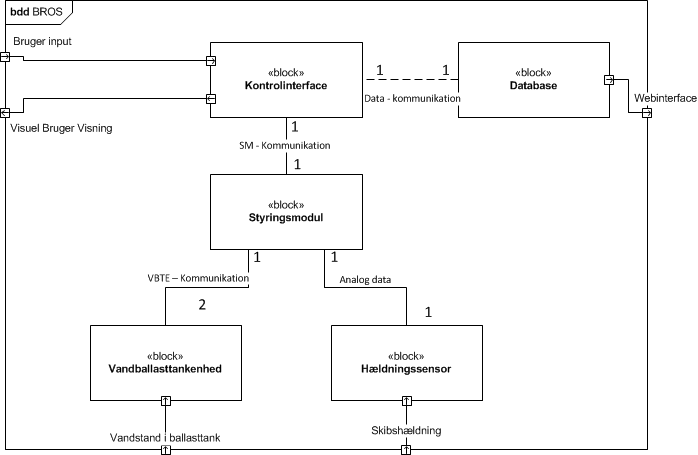
\includegraphics[scale=0.8]{billeder/Systemarkitektur/ibd_bros}
\caption{Internt blokdiagram for systemet}
\label{fig:idb_bros}
\end{figure}

Som det kan ses i figur anvendes der en række protokoller til kommunikation mellem systemets interne blokke. Disse protokoller skal defineres inden design og implementering af systemets blokke kan begynde.

Som eksempel vil der blive givet kommunikationsprotokollen mellem VBTE og Styringsmodulet som opskrevet i tabel \ref{tabel:protokoloversigt} med de indstillinger angivet \textit{\ref{tabel:forbindelsesindstillinger}}.


\begin{table}[H]
\centering
\begin{tabular}{|l|l|}
\multicolumn{2}{l}{{\Large Forbindelsesindstillinger}} \\\hline
Data Rate (kbps)&100\\\hline
VBTE1-Adressse&2\\\hline
VBTE2-Adresse&3\\\hline
Bytes sendt&1\\\hline
\end{tabular}
\caption{Forbindelsesinstillinger I2C}
\label{tabel:forbindelsesindstillinger}
\end{table}

\begin{table}[htbp]
\centering
\begin{tabular}{|l|l|p{10cm}|}
\multicolumn{2}{l}{{\Large Protokoloversigt}} \\\hline
%\hline
\textbf{Navn} &\textbf{Værdi} &\textbf{Beskrivelse}\\\hline
VBTENIVEAU&5&Sendes når SM ønsker at aflæse vandstandsniveauet\\\hline
TOPVENTIL&6&Sendes når VBTE skal åbne for topventilen (og dermed lukke for bundventilen)\\\hline
BUNDVENTIL&7&Sendes når VBTE skal åbne for bundventilen (og dermed lukke for topventilen).\\\hline
LUKVENTIL&8&Sendes når VBTE skal lukke for begge ventiler.\\\hline
\end{tabular}
\caption{Protokoloversigt for I2C}
\label{tabel:protokoloversigt}
\end{table}

Systemet er nu opdelt i fysiske blokke. For hver blok er der angivet et state machine. Kommunikationsprotokollen imellem blokkene er beskrivet. Designfasen kan påbegynde.




